\chapter{Design Analysis}
An algorithm is the idea behind a program. An algorithm can be implemented in multiple ways leading to varying performance and efficiency of the program, for example, using different data structures, data storage options i.e. if the data should be stored in memory or on file system, implementation language, library functions used etc. A design is a result of such numerous decisions which are made during the development process.  Very rarely is it possible to find the perfect design which would lead to a program performing with the same efficiency for the entire input space. Hence, while making the decisions it is important to evaluate the advantages and disadvantages of the chosen approach. This chapter is therefore dedicated to analyze the design choices made during the implementation. 

\section{Application of distributed computing}

As discussed in section \ref{sysMod}, the task submitted by the user to the master node is divided into sub-tasks and distributed among the slave nodes of the cluster. The slave nodes perform the allocated work and report the partial output which is merged at the master node. The flowchart \ref{lst:FC} summarizes the process. The \textit{MasterPrintingSoftware} follows the steps denoted in the left branch of the flow chart where as the \textit{SlavePrintingSoftware} follows the steps of denoted in the right branch of the flow chart. The \textit{MasterPrintingSoftware} and \textit{SlavePrintingSoftware} design decisions include:
\begin{enumerate}
\item Format of the sub-tasks allocated to the slaves nodes
\item Distribution of sub-tasks by the master
\item Format of the slave partial output 
\item Merging of the partial output 
\end{enumerate}

\begin{figure}
\centering
\begin{tikzpicture}[node distance=2.75cm] 
\node (start) [startstop] {Start};
\node (dec1) [decision,below of=start ,yshift=-0.75cm]{ Is master node?};
\node (Min1) [io, below left of=dec1 , xshift= -2cm] {Input main configuration file};
\node (Sin1) [io,below right of=dec1 , xshift= 2cm] {Receive sub-tasks from Master};
\node (Mpro1) [process, below of=Min1] {Parse Input, Create sub-tasks, Distribute Sub-tasks};
\node (Mpro2) [process, below of=Mpro1 ,yshift=-0.5cm] {Receive meta-data, compute full slice height, width, offset};
\node (Mpro3) [process, below of=Mpro2 ,yshift=-0.5cm] {Receive partial slices and merge to full slice};
\node (Mdec1) [decision,below of=Mpro3, yshift=-0.5cm]{ Is last slice?};
\node (Spro1) [process, below of=Sin1] {Perform computation and generate chunk-wise slices };
\node (Sdec1) [decision,below of=Spro1, yshift=-0.5cm]{ Is first chunk?};
\node (Spro2) [process, below left of=Sdec1,xshift= -1cm] {Send meta-data to the master};
\node (Spro3) [process, below of=Sdec1,yshift=-1cm ] {Send the partial slice to the master};
\node (Sdec2) [decision,below of=Spro3, yshift=-0.5cm]{ Is last chunk?};
\node (Mend) [startstop,below of= Mdec1 , yshift=-1.5cm] {End};
\node (Send) [startstop,below of=Sdec2, yshift=-1.25cm ] {End};

\draw [arrow] (start) -- (dec1);
\draw [arrow] (dec1) -| node {yes}(Min1);
\draw [arrow] (dec1) -| node {no}(Sin1);
\draw [arrow] (Min1) -- (Mpro1);
\draw [arrow] (Mpro1) -- (Mpro2);
\draw [arrow] (Mpro2) -- (Mpro3);
\draw [arrow] (Mpro3) -- (Mdec1);
\draw [arrow] (Mdec1.west) -|node {no} ++(-0.5,0)|-(Mpro3.west);
\draw [arrow] (Mdec1) -- node {yes}(Mend);
\draw [arrow] (Sin1) -- (Spro1);
\draw [arrow] (Spro1) -- (Sdec1);
\draw [arrow] (Sdec1) -| node {yes}(Spro2);
\draw [arrow] (Sdec1) -- node {no}(Spro3);
\draw [arrow] (Spro2) -| (Spro3);
\draw [arrow] (Spro3) -- (Sdec2);
\draw [arrow] (Sdec2.east)-|node {no} ++(0.5,0)|-(Spro1.east);
\draw [arrow] (Sdec2) -- node {yes}(Send);
\end{tikzpicture}
\caption{Distributed Printer Driver Flow Chart}
\label{lst:FC}
\end{figure}

Each of the design possible from the various combinations of the above decisions yields a different behavior of the component responsible for that particular task. The following sections describes the two designs implemented through the thesis in detail.  

\section{Prototype I- Input/Output using NFS }

Prototype I is the base prototype wherein the nodes communicate amongst each other the input and the partial output using the shared network file system. The synchronization amongst the nodes is done via message passing. 

\subsection{Master sub-task creation and distribution}
User submits the job to the master node using a configuration file in \textit{JSON} format. The JSON document contains a member called as \textit{PrintObjectFiles} whose member values indicate the geometry, texture, orientation etc of the object to be printed. The \textit{FileParserPJ} component of \textit{MasterPrintingSoftware} parses the input and converts it into an internal mesh representation called as the print object, with each having it's own unique identifier. The print objects are grouped together into a print job. Each print job is the organized in the print tray and then passed to the \textit{MasterDistributor} component which is in charge of sub-task creation and distribution. The sub-tasks distributed by the component can be already created print jobs or they can be in the same format as the received input i.e. configuration file. In this prototype, the \textit{MasterDistributor} creates a configuration file for each slave with the exactly same format as the configuration file parsed by the \textit{FileParserPJ} with a few changes i.e. the \textit{PrintObjectFiles} contains details of only the print models allocated to that particular slave and the \textit{OutputFolder} value is the folder location for the slave to write the partial output. In the figure \ref{fig:MasterConfigurationFile}, the configuration file received by the master node has the \textit{PrintObjectFiles} containing four inputs models which are distributed by the master as seen in the figure \ref{fig:Slave1ConfigurationFile} for the slave with rank 1 and figure \ref{fig:Slave2ConfigurationFile} for slave with rank 2. 

\begin{figure}[ht!]
\centering
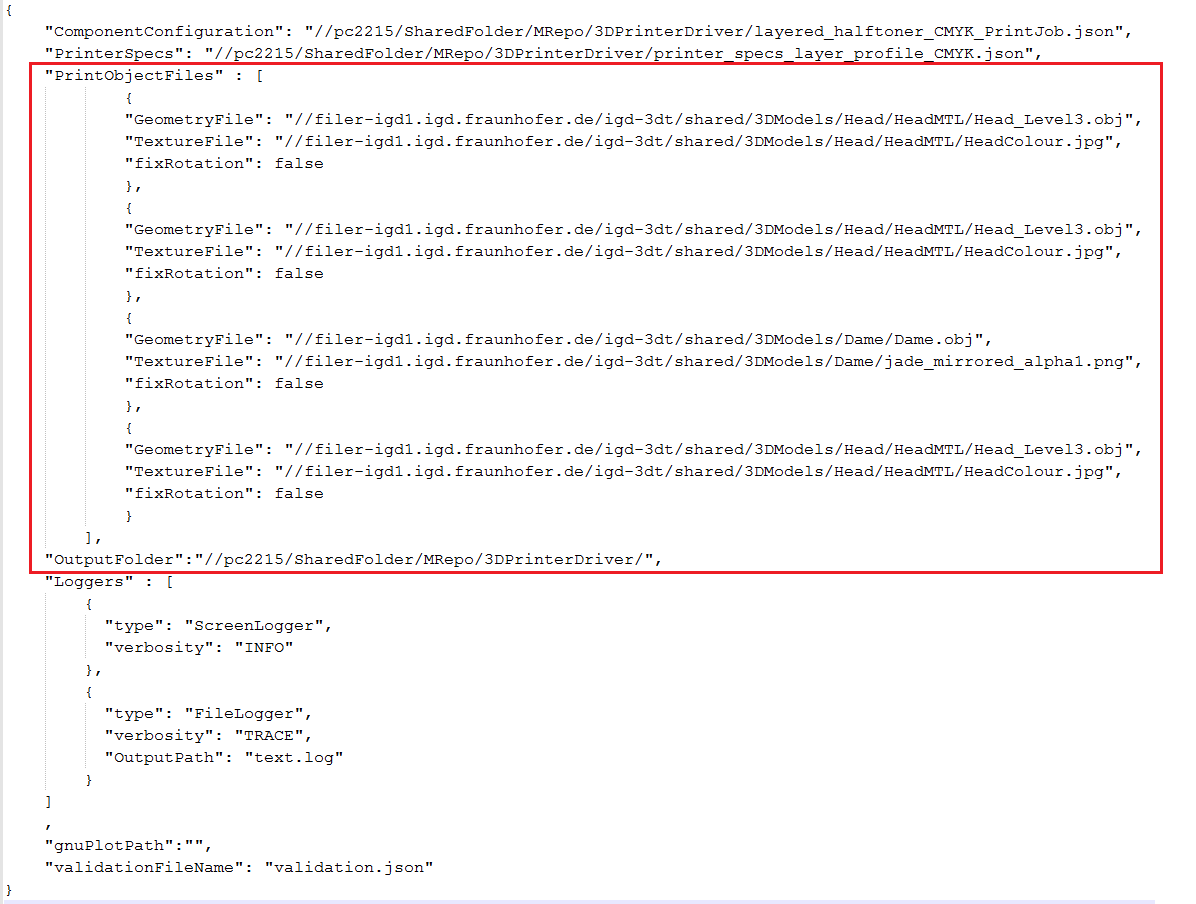
\includegraphics[scale=0.75]{MasterConfigurationFile.png}
\caption{Master Configuration file}
\label{fig:MasterConfigurationFile}
\end{figure}

\begin{figure}[ht!]
\centering
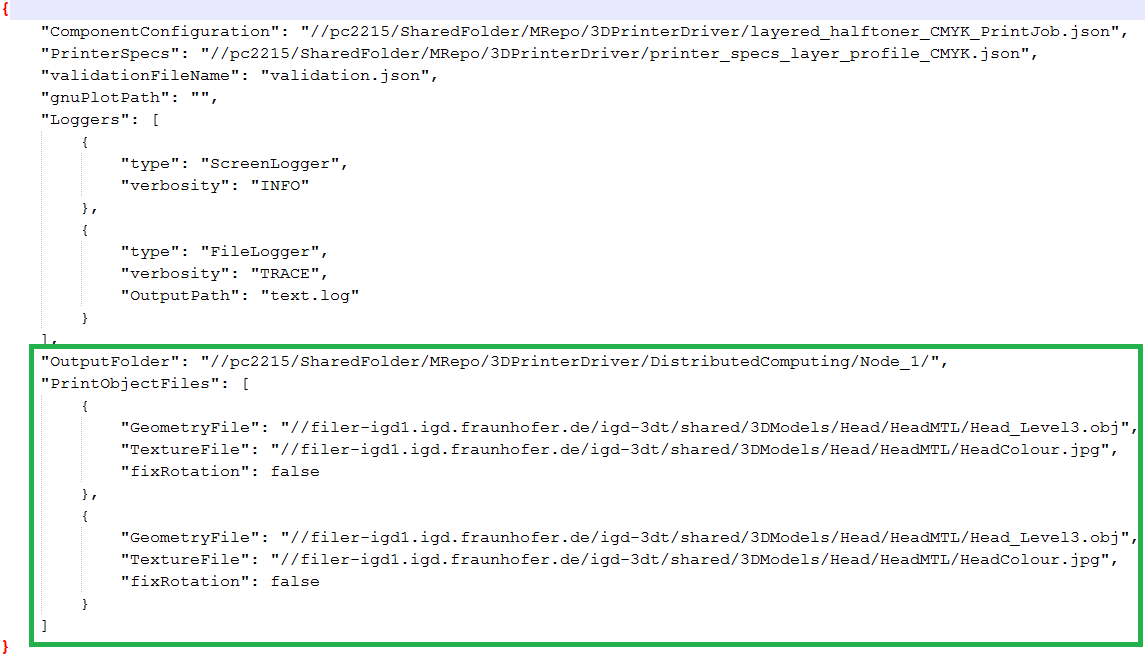
\includegraphics[scale=0.75]{Slave1ConfigurationFile.png}
\caption{Slave 1 Configuration file}
\label{fig:Slave1ConfigurationFile}
\end{figure}

\begin{figure}[ht!]
\centering
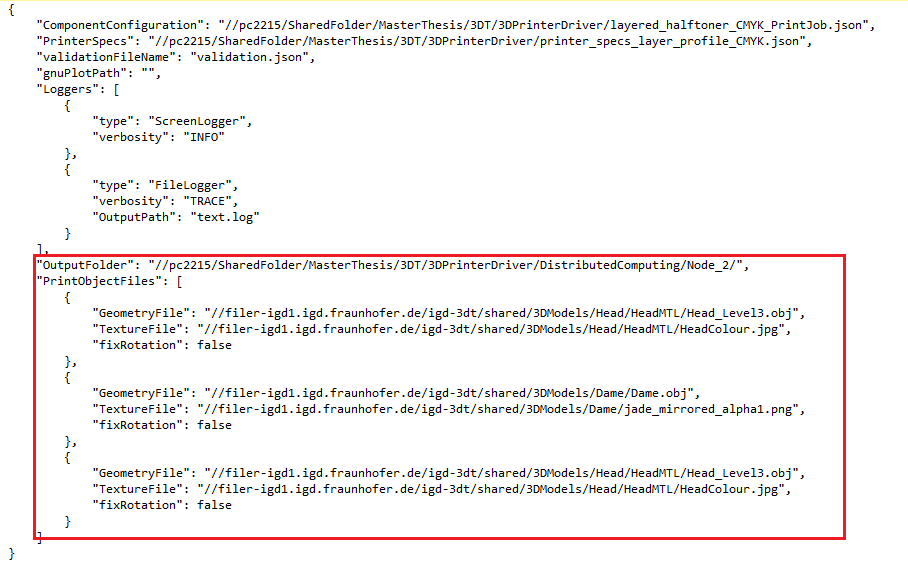
\includegraphics[scale=0.75]{Slave2ConfigurationFile.png}
\caption{Slave 2 Configuration file}
\label{fig:Slave2ConfigurationFile}
\end{figure}

This prototype is possible only if the cluster nodes have read/write permission to the shared network file system where the geometry, texture files and input/output folders are stored /created. The \textit{MasterDistributor} creates a unique path for each slave using the rank of the slave and writes the configuration file to this path. It then communicates to the slave only the path where the slave can find the configuration file. The sequence diagram in the figure \ref{fig:SequenceDiagram1} summarizes the communication between the master and the slaves.  

\begin{figure}[ht!]
\centering
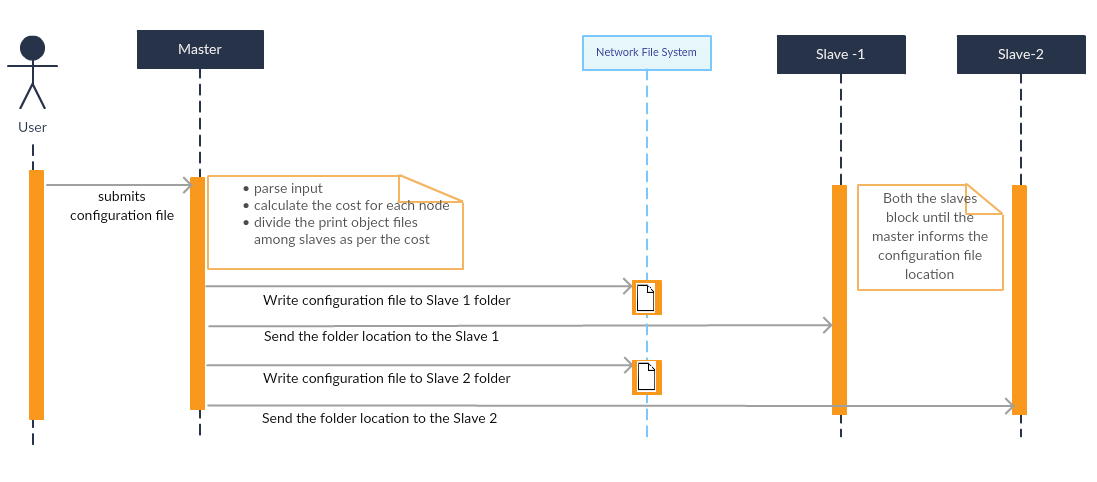
\includegraphics[scale=0.6]{SequenceDiagram1.png}
\caption{Master-slave input communication}
\label{fig:SequenceDiagram1}
\end{figure}

The pros of distributing the sub-tasks through the configuration file are:
\begin{itemize}
\item \textbf{Design simplicity}: The most important aspect of this design is it's simplicity as the \textit{SlavePrintingSoftware} pipeline does not need to be modified greatly which means that it is almost similar to running a single instance of the non-distributed version of the 3D Printing pipeline. 
\item \textbf{Lower Communication Overhead}: Slave nodes are blocked until the master communicates the configuration file path to each slave. Communication of the file path is faster as it is less number of bytes to be exchanged among the nodes as compared to the number of bytes to be sent when print jobs are distributed .
\item \textbf{Faster Disk I/O}: The configuration file read and writes i.e. disk I/O (both at the master and slave) are much faster than sending the print job as series of bytes. It is simpler implementation as communicating the print jobs as series of bytes would require defining a protocol for packing and unpacking of the print jobs with an additional effort of performing the packing at master and unpacking at the slave nodes.
\item \textbf{No serialization and deserialization}: As the configuration files are in JSON format, there are very efficient library functions which allow to read and write the files with ease. As the format of the files is very standard, there is no need for serialization and deserialization of the files even if the nodes have varying underlying system architecture.        
\end{itemize}

The cons of distributing the sub-tasks via configuration file are: 
\begin{itemize}
\item \textbf{Dependency on shared network file system}: This prototype has a strong requirement that the nodes have a shared network file system and each node must have read access to the model texture/geometry file along with write access to the output folder to dump the partial output. If the print jobs are communicated as stream of bytes, it is possible to get rid of this requirement.
\item \textbf{Performance overhead}: The configuration file, model geometry and texture files are parsed twice, once by the master to create the prints jobs needed for cost computation and once by the slaves for actual computation. This leads to redundant execution of the \textit{FileParserPj} and \textit{PrintJobOrganizer} at both master and slave nodes which accumulates to a significant performance overhead.
\item \textbf{Disk I/O performance limited by network bandwidth}: As the files are read and written to the shared network file system, the network bandwidth limits the speed of the disk I/O. With increase in number of slave nodes, the load at the master to write the configuration file per slave increases which may become a performance bottleneck. 
\end{itemize}

\subsubsection{Sub-Task Distribution}

The sub-tasks are distributed by the \textit{MasterDistributor} component based on a cost function. The goal of the distribution is to allocate equal work to each slave i.e. none of the slaves are over-worked and all of them finish the work almost at the same time. One of the main reasons which makes it important to achieve load balancing is to ensure better utilization of the cluster resources, a cluster as a whole will perform well only if each of the nodes do equal work leading to none of the nodes being the bottleneck. 

The cost function used for distribution of the tasks evaluates the cost of each work item and allocation of work item among the slave nodes is done such a way that total cost of allocated work items is equal for each node. The cost for each work item may vary depending on the work item, for example for print objects, the size or the print volume of the print objects could be seen as cost of the work item, or priority assigned to the print objects can be another way to evaluate the cost. 
\newline
\textbf{Naive cost function implementation }\newline
Each print object \begin{math}O_{i}\end{math} has a bounding box. The minimum bounding box (\begin{math}b_{min}^i\end{math}) and maximum bounding box(\begin{math}b_{max}^i\end{math}) is calculated. Using \begin{math}b_{min}^i\end{math} and \begin{math}b_{max}^i\end{math}, the width(\textit{w}), height(\textit{h}), and length(\textit{l}) of each print object is calculated as per equation \ref{eq:length}

\begin{equation}
\label{eq:length}
\begin{aligned}
w=(b_{max}^i).y-(b_{min}^i).y \\
h=(b_{max}^i).z-(b_{min}^i).z \\
l=(b_{max}^i).x-(b_{min}^i).x \\
\end{aligned}
\end{equation}

The volume (\begin{math}V^i\end{math}) of the print object \begin{math}O_{i}\end{math} is calculated using the equation \ref{eq:volume}.

\begin{equation}
\label{eq:volume}
V^i= w*h*l
\end{equation}

The total sum of the volumes of \textit{k} print objects calculated using equation \ref{eq:Sum} 

\begin{equation}
\label{eq:Sum}
Total Volume =\sum\limits_{i=1}^{k}{V^i}
\end{equation}

Threshold (for each node in a cluster of size \textit{n-1}) calculated using equation \ref{eq:threshold} is used for allocating the sub-tasks to the slaves. The cluster size considered is \textit{n-1} as the master is not allocated any sub-task and is hence excluded from the cluster of slaves.

\begin{equation}
\label{eq:threshold}
Threshold =(\sum\limits_{i=1}^{k}{V^i})/(n-1)
\end{equation}

The allocation of the sub-tasks is done using the greedy approach. The list of volumes calculated using equation \ref{eq:volume} is sorted in the  descending order. Then the allocation of the object is done in a round-robin fashion to each slave  until the allocated total volume  for the node is greater than or equal to the threshold. If the threshold is already reached for the node, then the node is skipped. The allocation of the print object stops when each node\textquotesingle s capacity has been consumed or all the print objects are assigned. The listing \ref{lst:ppga} summarizes the distribution logic.

\begin{lstlisting}[language=C++,label={lst:ppga},caption={Distribute Tasks- Greedy Approach}]
DistributeTasks(VolList,threshold,NumNodes)
{
	std::sort(VolList.begin(), VolList.end(),std::greater<>()); // sort in descending order
	int listOfSum(NumNodes-1)={0};
	int vlSize= VolList.size();
	int nodeInd= 1;
	int allocatedIndexList(NumNodes-1);
	for (size_t ind = 0; ind < vlSize;)
	{
			if (listOfSum[nodeInd] < threshold)
			{
				sumList[nodeInd] = sumList[nodeInd] + tempList[ind];
				indList[nodeInd].push_back(ind);
				ind++;
			}
			
			if (nodeInd == NumNodes-1)
				nodeInd = 0;
			else 
				nodeInd++;
	}
}
\end{lstlisting}

This greedy approach is known to give a \begin{math} \frac{7}{6} \end{math}-approximation to the optimal solution of the optimization version \cite{pp2016}.

\subsection{Slave Partial Output}

The \textit{SlaveReporter} component receives the container of \textit{slices} whose size is equal to the \textit{chunk} size, as input from the previous component in the pipeline. At each of the slaves, the container actually contains the partial \textit{slices} which are sent to the master for merging.  Each slice internally stores the width, height and the buffer which contains the material id of the assigned material at varying \textit{(x,y)} coordinate. As the cluster may contain heterogeneous machines with varying system architecture, to ensure proper interpretation of the slices at the master, the slices are serialized. \textit{Serialization} of the slices includes serializing the width, height (unsigned integers to same size), buffer to an output stream (std::ostream). The behavior of the \textit{SlaveReporter} component is summarized in the figure \ref{fig:SlaveReporterActivityDiagram}. \newline
\begin{figure}[ht!]
\centering
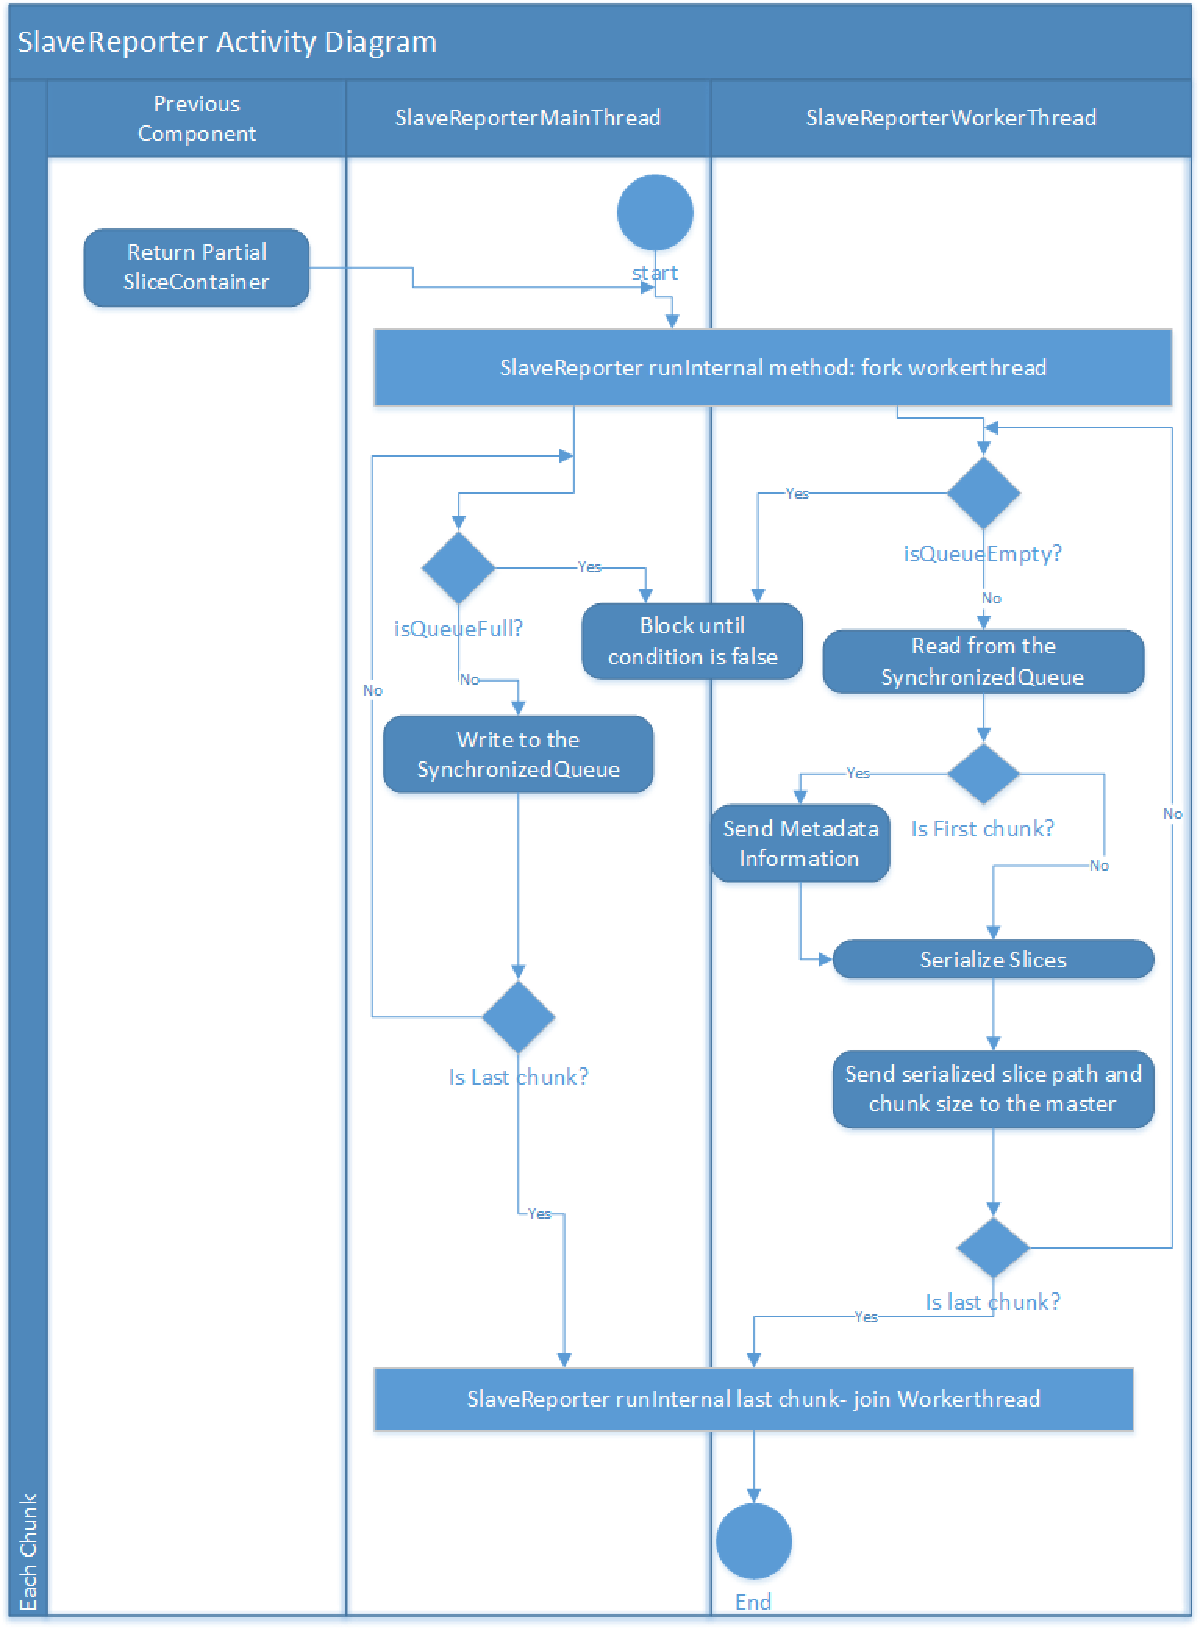
\includegraphics[scale=0.8]{SlaveReporterActivityDiagram.PNG}
\caption{\textit{SlaveReporter} Activity Diagram}
\label{fig:SlaveReporterActivityDiagram}
\end{figure}

\textbf{Analysis of component behavior} \newline

The \textit{SlaveReporter} component is multi-threaded and uses a synchronized queue for inter-thread communication. The \textit{runInternal} method of each component is the main thread of execution i.e. the cuttlefish process, whereas in the first run of this method a worker thread is created which executes asynchronously to perform certain tasks. The main thread interacts with the other components whereas the worker thread interacts only with the main thread and worker threads of \textit{MasterPrintingSoftware-MasterMerger} component. \newline
The interaction between the main thread and the worker thread can be viewed as the classic producer consumer problem, see figure \ref{fig:ProducerConsumerProblem}, where in the main thread produces the partial slices which are consumed by the worker thread and serialized. Each chunk of partial slices is one work item produced by the main thread and inserted in the buffer. Depending on the type of buffer, there might be varying number of synchronization points between the threads. In the current design, the buffer is implemented as a queue of limited size i.e. a bounded buffer. As the buffer is of fixed size, there are two conditions which lead to blocking either the main thread or the worker thread. As the main thread acts as the producer, it blocks when the buffer is full (i.e. slow consumer) and waits on a condition indicating at least one free slot. The worker thread acts as the consumer and blocks when there is no work item to consume and waits until there is at least one full slot. \newline

\begin{figure}[ht!]
\centering
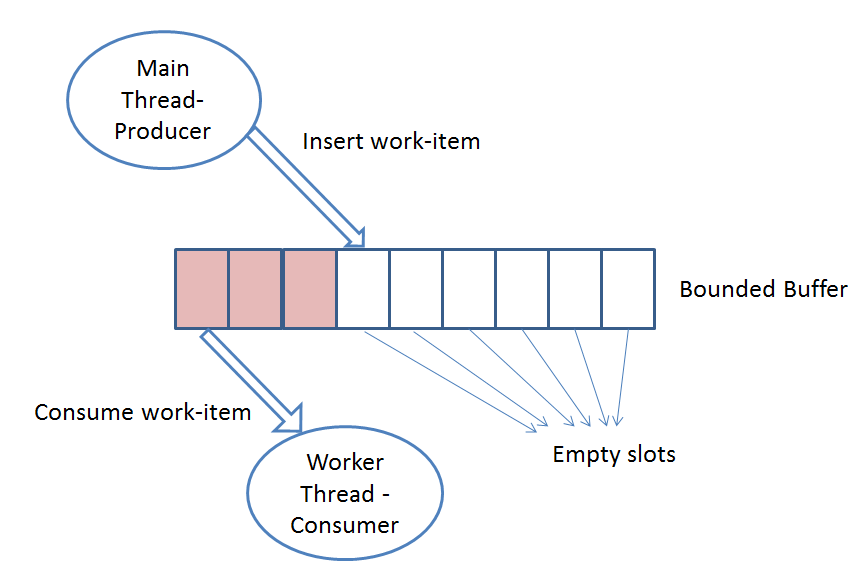
\includegraphics[scale=0.6]{ProducerConsumerProblem.PNG}
\caption{Producer-Consumer Problem}
\label{fig:ProducerConsumerProblem}
\end{figure}

The worker thread performs the task of serialization and once each chunk of slices is serialized it communicates with worker thread of \textit{MasterPrintingSoftware-MasterMerger} component the chunk size- it acts as a way of synchronization of the worker threads between the components. The worker thread sends some meta-data  only for the first chunk of slices which includes slice height, slice width, chunk size, total number of slices. This meta-data is used by the main thread of \textit{MasterPrintingSoftware-MasterMerger} component for creating full slices.

The pros of \textit{SlaveReporter} component design:
\begin{itemize}
\item \textbf{Separation of concerns}: The main thread is responsible for assigning the work to the worker thread and returns to continue with execution of the pipeline with the next chunk whereas the worker thread is responsible for communication and serialization.  
\item \textbf{Asynchronous communication}: The worker thread performs the blocking calls for synchronization with worker threads of \textit{MasterPrintingSoftware-MasterMerger} component. As it does so asynchronously, the communication never leads to blocking the main thread. Both the main thread and worker thread execute in parallel.
\end{itemize} 

The cons of \textit{SlaveReporter} component design:
\begin{itemize}
\item \textbf{Synchronization Overhead}: The main thread and the worker thread need to synchronize access to the shared buffer so as to avoid race condition along with blocking calls on buffer full/ empty condition. The size of the buffer influences the performance of the solution i.e. if unlimited buffer is used the producer will never block whereas if no buffer is used there is no need for explicit synchronization as producer produces only one item and the consumer consumes it after it is produced.
\item \textbf{Increased implementation complexity}: Synchronization between the threads leads to added implementation complexity and if not managed properly might lead to deadlock. 
\end{itemize} 

\subsection{Partial Output Merging at Master} 

The partial slices serialized by the slaves are de-serialized at the \textit{MasterMerger} component. The \textit{MasterMerger} component creates worker thread per slave node in the cluster which interacts with the worker thread created by the \textit{SlaveReporter} component. The main thread of the \textit{MasterMerger} component synchronizes with worker threads at various points during the execution. The worker threads of \textit{MasterMerger} component first wait to receive the meta-data information from the \textit{SlaveReporter} component worker thread. After they have received the slice height, width, total number of slices and chunk size, they synchronize with the main thread and indicate the receipt of the meta-data. The worker threads then wait to receive the chunk size of the serialized data from the worker threads of \textit{SlaveReporter} component, the receipt of the chunk size is the indication that slices are serialized and ready for deserialization. On receiving the chunk size, they start with deserialization of the slices and create a container of deserialized partial slices. \newline

In the meantime, the main thread uses the received meta-data information to calculate the full slice height, width, total number of slices and chunk size for the full slices and then creates the container of the full slices. The worker threads at the master node continue to deserialize the chunk they received from the slaves and block until the container of full slices is created by the main thread and ready to be written. On signaling of availability of the container by the main thread, the worker thread then proceed with writing the partial slices to the full slices. \newline

Each worker thread has a dedicated section in the full slice where it writes to, which helps to avoid write-write conflicts on the shared data structure. The main thread waits until all the worker threads have finished writing the partial slices to the full slices and has container of full slices with earlier calculated chunk size ready. The main thread then continues to proceed with the pipeline with fully merged slices whereas worker threads continue to deserialize the slices or communicate with worker threads of the slave or write the partial slices to the full slice in the container provided by the main thread. The activity diagram \ref{fig:MasterMergerComponent} shows the activity of the main thread and worker threads of \textit{MasterMerger} component. 
   
The main thread at the master computes the slice height, slice width, offset for each worker thread and total number of slices. The slice height is computed as the addition of all the partial slice heights. If the full slice height is exceeding the print bed height, then full slice height is set to the print bed height. The height is calculated as the addition of partial slice heights because the partial slices from the slaves are written one below the other in y-axis until either the print bed height is reached or each of the slave node partial slices are placed. If the print bed height is reached and there are still pending slave partial slices to be fit in the full slice, then the maximum partial slice width is taken as the x-offset and the remaining slices are then places along the y-axis again with each having the x-offset. The listing \ref{lst:fsh} summarizes the logic of full slice height calculation.

\begin{lstlisting}[language=C++,label={lst:fsh},caption={Calculate full slice height}]
int fullsliceHt(std::vector<int> listOfpartilSliceHt)
{
	int maxAllowedHt = getPrintBedHeight(); // get the print bed height
	int totalht(0);
	for(size_t i =0;i<listOfpartilSliceHt.size(),i++)
	{
		totalht =  listOfpartilSliceHt[i] + totalHt;
	}
	if(totalht > maxAllowedHt)
	{
		totalHt= maxAllowedHt; 
		m_xOffsetNeed=true; // to indicate that x-offset will be added to some slaves
	}
	return 	totalHt;
}

\end{lstlisting}

The full slice width is calculated as the maximum of the all the partial slice widths. If the total height calculated exceeds the print bed height, then total slice width is calculated as the sum of all slice widths. If the total slice width crosses the print bed width, then there is no way to fit all the partial slices in the given print bed and hence some of the slaves need to be dropped otherwise the full slice width is equal to the sum of individual partial slice widths. The full slice width calculation is summarized in the listing \ref{lst:fsw}     


\begin{lstlisting}[language=C++,label={lst:fsw},caption={Calculate full slice width}]
int fullsliceWd(std::vector<int> listOfpartilSliceWd)
{
	int maxAllowedWd = getPrintBedWidth(); // get the print bed width
	int totalWd(0);
	if(m_xOffsetNeed) // this is set to true if the total sum of slice heights > print bed height.
	{
		for(size_t i =0;i < listOfpartilSliceWd.size(),i++)
		{
			totalWd =  listOfpartilSliceWd[i] + totalWd;
		}
		if(totalWd > maxAllowedWd)
		{
			m_DropSlaves=true; // to indicate that some slaves need to be dropped
		}
	}
	else
	{
		for(size_t i =0;i < listOfpartilSliceWd.size(),i++)
		{
			totalWd = totalWd > listOfpartilSliceWd[i]? totalWd : listOfpartilSliceWd[i];
		}
	}
	return 	totalWd;
}
\end{lstlisting}

The total number of full slices is the maximum value from the received total number of slices from the slaves. The main thread needs to keep track of the individual total number of slices from each slave node so as to ensure that the master does not block for a worker thread to write to the full slices when there are no more partial slices left. 

\begin{figure}[ht!]
\centering
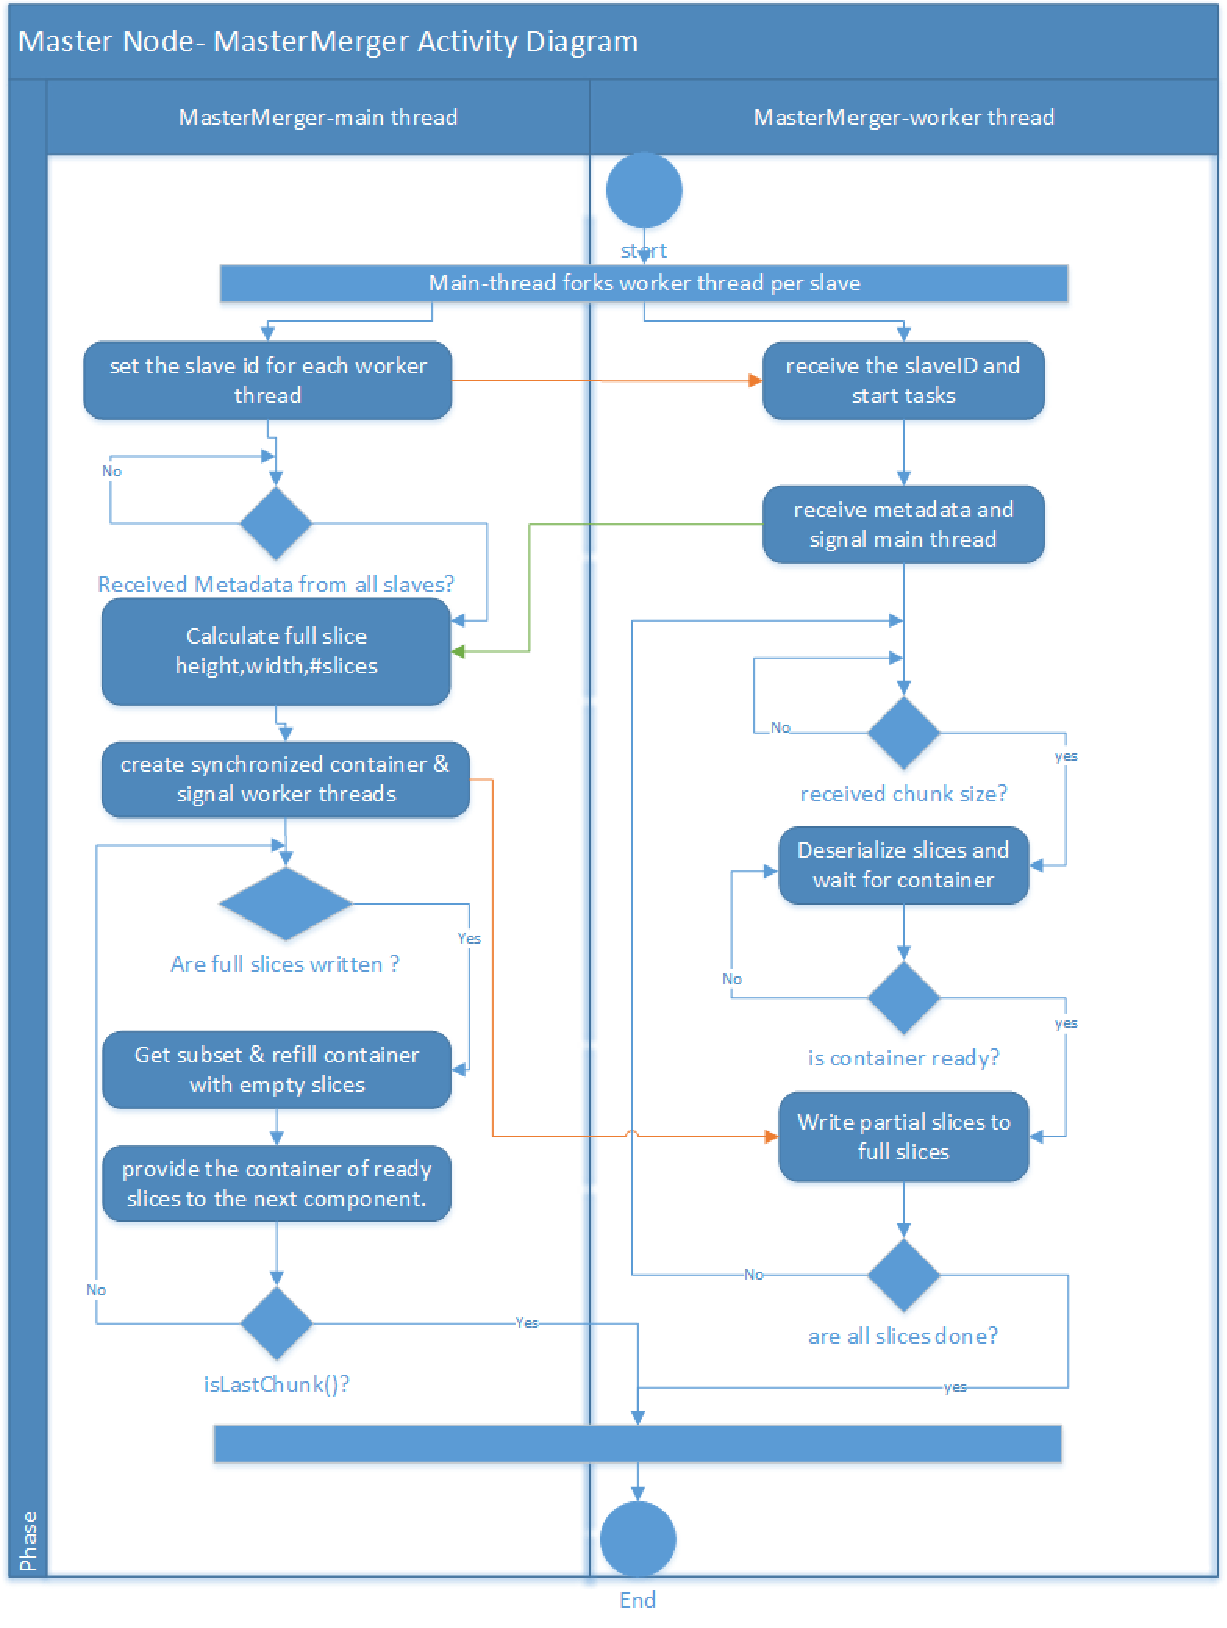
\includegraphics[scale=0.85]{MasterMergerComponent.PNG}
\caption{\textit{MasterMerger} Component- Activity Diagram}
\label{fig:MasterMergerComponent}
\end{figure}

The slice container to be provided by the main thread is a synchronized slice container which means that while removing the individual slices or subset of slices or adding the slices to the container, each thread needs to obtain the lock over the container and modify the container thereafter. The use of synchronized container ensure no data race on the shared data structure. \newline 

The pros of the \textit{MasterMerger} component design are:  
\begin{itemize}
\item Asynchronous communication: The worker threads for each slave node communicate with the worker thread of the SlaveReporter component asynchronously without blocking the execution of the main thread. This also helps to maintain the separation of the responsibilities among the worker threads as each worker thread is responsible it assigned slave node.
\item Exploiting the possible parallelism: The worker threads perform deserialization of partial slaves and write to their assigned section of the full slices simultaneous without write-write conflicts amongst them. The main thread also continues to work on computing the full slice height, width etc while the worker threads are deserializing and when the worker threads are done writing to the full slice container, return the full slice conatiner and proceed with next pipeline component execution in a chunk-wise fashion. This design maintains the streaming architecture of the original non-distributed version of the pipeline. 
\end{itemize}

The cons of the \textit{MasterMerger} component design are:
\begin{itemize}
\item Synchronization Overhead: As there are many synchronization points during the execution where either the worker threads block or the main thread block, it might lead to overhead in the execution run time. Also the synchronization leads to added code complexity. 
\item Limited possibilities of partial slice arrangement: As the arrangement of the partial slices in the full slices is done, there is a possibility of not achieving the optimal arrangement leading to the wastage of the print area along with incapability of accommodating each slave. This might lead to dropping one or more slaves from the merging process to enable making the best possible use of the work done by the slaves.  
\item Possibility of deadlock: The main thread at the master blocks until each slave has received the meta-data or written to the full slices. The main thread might remain blocked if one of the slaves crashes which will eventually lead to a deadlock as other slaves might get blocked until the main thread refills the container with new full slices. To avoid this, use of timeouts could be done. If the worker thread for a particular slave does not respond within the timeout period, then slave could be dropped. The timeouts shouldn't be too small leading unnecessary dropping of the slaves or too long leading to increased execution time overhead. The use of timeouts adds further code complexity.
\end{itemize}

\section{Prototype II- Input/Output independent of NFS }





